% -*- Mode: LaTeX; tab-width: 4 -*-
%
% Work on Sheldon Axler 'Linear Algebra Done Right'.
% Pedro Crespo Valero - 2015, 2021

%%%%%%%%%%%%%%%%%%%%%%%%%%%%%%%%%%%%%%%%%%%%%%%%%%%%%%%%%%%%%%%
\newpage
\section{Eigenvalues and Eigenvectors}
%------------------------------------------------------------------------ 
\subsection*{Summary}
\begin{description}
\item For an operator $T\in\mathcal{L}(V)$ and $U$ a subspace of $V$, we say that $U$ is \textbf{invariant} under $T$ if $\forall u\in U \implies Tu\in U$.
\item $U$ is invariant under $T$ if $T|_U$ is an operator on $U$.
\item $\{0\}$, $V$, $\nullspace{T}$ or $\rangespace{T}$ are invariant under $T$.
%
\item A scalar $\lambda\in \mathbf{F}$ is an \textbf{eigenvalue} of $T\in\mathcal{L}(V)$ if there exists a non-zero vector $u\in V$, denoted \textbf{eigenvector}, such that $Tu=\lambda u$.
\item $T$ has a one-dimensional invariant subspace $\iff$ $T$ has an eigenvalue
\item $Tu = \lambda u \iff (T-\lambda I)u=0$. [Any non-zero vector in $\nullspace{(T-\lambda I)}$ is an eigenvector of $T$ associated to $\lambda$]
\item $\lambda$ is an eigenvalue of $T$ iff
\begin{itemize}
\item $(T-\lambda I)$ is \textbf{non}-injective (i.e. $0$ is not the only vector in $\nullspace{(T-\lambda)}$
\item $(T-\lambda I)$ is \textbf{non}-invertible (so the trivial solution is not the only solution)
\item $(T-\lambda I)$ is \textbf{non}-surjective
\end{itemize}
\item The sets of eigenvectors of $T$ corresponding to $\lambda$ equal $\nullspace{(T-\lambda I)}$ and therefore this set is a subspace of $V$.
%
\item[T6] If $\lambda_1,\cdots,\lambda_m$ are distinct eigenvalues of $T$ and $v_1,\cdots,v_m$ are corresponding non-zero eigenvectors, then $(v_1,\cdots, v_m)$ is linearly independent. 
%
\item[C9] Each operator on $V$ has at most $\dimension{V}$ distinct eigenvalues
%
\item $\mathcal{P}(\mathbf{F})\to \mathcal{L}(V)$ and $p \rightsquigarrow p(T)$ linear map
\begin{itemize}
\item $T^m = T\cdots T$ with $T^mT^n = T^{m+n}$
\item $p(T)=a_0I+ a_1 T+ \cdots + a_m T^m$
\item Conmutative $(pq)(T) = p(T)q(T) = (qp)T = q(T)p(T)$
\end{itemize}  
\item[T10\label{itm:T5_10}] Every operator on a finite-dimensional, non-zero \emph{complex} vector space has an eigenvalue.
%
\item Goal: Given an operator $T\in\mathcal{L}(V)$, there exists a basis of $V$ with respect to which $T$ has a reasonably simple matrix $\mathcal{M}(T)$ (i.e. as many zeros as possible).
\item By T10, any complex vector space has at least one eigenvalue $\lambda$. Then extending a list of an autovector $(v)$ to a basis of V results in a matrix like
\begin{align*}
\begin{bmatrix}
\lambda &&  && \\
0  && *  && \\
\vdots && &&  \\
0 &&  && 
\end{bmatrix}
\end{align*}
since $Tv = \lambda v$.
\item[P12] $T\in\mathcal{L}(V)$ and the list $(v_1,\cdots,v_n)$ a basis of $V$. The following are equivalent:
\begin{itemize}
\item $\mathcal{M}(T,(v_1,\cdots,v_n))$ is upper triangular.
\item $Tv_k\in\mathrm{span}(v_1,\cdots,v_k)$ for each $k=1,\cdots, n$.
\item Each $\mathrm{span}(v_1,\cdots,v_k)$ is invariant under $T$ for each $k=1,\cdots, n$. See how subspaces of increasing dimension are invariant
\begin{align*}
\begin{bmatrix}
y_1\\
0 \\
0 \\
\vdots
\end{bmatrix}
\begin{bmatrix}
y_1\\
y_2 \\
0 \\
\vdots
\end{bmatrix}
\cdots =
\begin{bmatrix}
\lambda_1 &  & & * \\
  & \lambda_2  & \\
  &  & \ddots & \\
0 & &        & \lambda_n
\end{bmatrix}
\begin{bmatrix}
x_1\\
0 \\
0 \\
\vdots
\end{bmatrix}
\begin{bmatrix}
x_1\\
x_2 \\
0 \\
\vdots
\end{bmatrix}
\cdots
\end{align*}
\end{itemize}
Notice that we refer to $Tv_1 \in \mathrm{span}(v_1)$, $Tv_2 \in \mathrm{span}(v_1, v_2)$, $\cdots$

\item[T13] $V$ complex vector space and $T\in\mathcal{L}(V)$, then $T$ has an upper-triangular matrix with respect to some basis of $V$

\item Suppose $T\in\mathcal{V}$ has an upper-triangular matrix with respect to some basis of $V$. Then
\begin{itemize}
 \item[P16] $T$ is invertible $\iff$ the entries of the diagonal of that upper-triangular matrix are nonzero
 \item[P18] The eignevalues of $T$ are precisely the entries of the diagonal of that upper-triangular matrix.
\end{itemize}

\item[P20] If $T\in\mathcal{L}(V)$ has $\dimension{V}$ distinct eigenvalues, then $T$ has a diagonal matrix with respect to some basis of $V$

\item[P21\label{itm:P5_21}] $T\in\mathcal{L}(V)$ and $\lambda_1,\cdots,\lambda_m$ distinct eignevalues of $T$.
\begin{itemize}
\item $T$ has a diagonal matrix with respect to some basis of $V$
\item $V$ has a basis consisting of eigenvectors of $T$
\item exists one-dimensional subspaces $U_1,\cdots,U_n$ of $V$, each invariante in $T$ and $U_1\oplus\cdots\oplus U_n$
\item $V=\nullspace{(T-\lambda_1I)}\oplus\cdots \oplus\nullspace{(T-\lambda_mI)}$
\item $\dimension{V}=\dimension{\nullspace{(T-\lambda_1I)}}+\cdots+ \dimension{\nullspace{(T-\lambda_mI)}}$
\end{itemize}
Notice $\dimension{V}=n$ and $m\leq n$ is the number of distinct eigen-values.

\item[T24] Every operation on a finite-dimensional, nonzero, \emph{real} vector space has an \emph{invariant} subspace of dimension 1 or 2.

\item[Projection Operator\label{itm:D5_projection_operator}] $P_{U,W}\in\mathcal{L}(V)$ is the projection onto $U$ with $\nullspace{P} = W$ and provided that $V=U\oplus W$, then
\begin{itemize}
\item $\forall v\in V$ we can express $v=u+v=P_{U,W}v+P_{W,U}v$
\item ${P_{U,W}}^2 = P_{U,W}$
\item $\rangespace{P_{U,W}}=U$ and $\nullspace{P_{U,W}}=W$
\end{itemize}

\item[T26] Every operator on an \emph{odd}-dimensional \emph{real} vector space has at least an eigenvalue.

\end{description}

%------------------------------------------------------------------------ 
\subsection*{Exercises}
\setcounter{paragraph}{0}

%------------------------------------------------------------------------ 
\exo{}Any element $u\in \sum U_i$ can be written as a sum $u = u_1 + \cdots + u_n$ with $u_i\in U_i$. Using additivity of the operator  $T\in\mathcal{L}(V)$
\begin{align*}
Tu = T(\sum u_i) = \sum Tu_i = Tu_1 + \cdots T u_n
\end{align*}
but $Tu_i\in U_i$ since $U_i$ is invariant under $T$. Therefore $Tu\in \sum U_i$ and $\sum U_i$ is invariant under $T$ as well.
%------------------------------------------------------------------------ 
\exo{} $\forall u\in \cap U_i$ implies $u\in U_i$ then, since $U_i$ is invariant under $T$, $Tu\in U_i\subseteq\cap U_i$ which demonstrates that $\cap U_i$ is also invariant under $T$.
%------------------------------------------------------------------------ 
\exo{} 

%------------------------------------------------------------------------ 
\exo{} $\forall u\in\nullspace{(T-\lambda I)} \implies (T-\lambda I)u = 0$
\begin{align*}
Tu=\lambda u \\
STu =S(\lambda u) = \lambda Su \\
TSu = \lambda Su \\
(T-\lambda I) Su = 0 
\end{align*}
which demonstrates that $Su\in\nullspace{(T-\lambda I)}$ and hence $\nullspace{(T-\lambda I)}$ is invariant under $S$.
%------------------------------------------------------------------------ 
\exo{}Let $u=(u_1,u_2)\in \mathbf{F}^2$, then we use the condition $Tu=\lambda u$:
\begin{align*}
T(u_1,u_2) = (u_2, u_1) = \lambda(u_1,u_2)
\end{align*}
which is satisfied if
\begin{align*}
u_2 = \lambda u_1 \\
u_1 = \lambda u_2
\end{align*}
or $u_2 = \lambda u_1 = \lambda^2 u_2$ that results in $\lambda=\pm 1$ provided that $v_2\neq 0$. Therefore for $\alpha\in \mathbf{F}$, vectors as $\alpha(1,1)$ are solutions with $\lambda=1$ and the vectors $\alpha(1,-1)$ are associated to $\lambda = -1$ \footnote{notice that $(1,-1) \propto (-1,1)$ since $\alpha\in \mathbf{F}$}. Let us verify that these are eigen-vectors/values:
\begin{align*}
T(\alpha,\alpha) = (\alpha,\alpha) \\
T(\alpha,-\alpha) = (-\alpha,\alpha) = -1(\alpha,-\alpha)
\end{align*}

%------------------------------------------------------------------------ 
\exo{} $T(v_1,v_2,v_3) = \lambda (v_1,v_2,v_3)$ leads to
\begin{align*}
2v_2 = \lambda v_1 \\
0 = \lambda v_2 \\
5v_3 = \lambda v_3
\end{align*}
From the third equation $\lambda=5$ provided $v_3\neq 0$. For $\alpha \in \mathbf{F}$, vectors as $(0,0,\alpha)$ are eigenvectors associated to $\lambda=5$. Let us verify it: $T(0,0,\alpha) = (0,0,5\alpha) = 5(0,0,\alpha)$.

%------------------------------------------------------------------------ 
\exo{} $Tv = \lambda v \iff \mathcal{M}(T)\mathcal{M}(v) = \lambda \mathcal{M}(v) \iff \mathcal{M}(T -\lambda I) \mathcal{M}(v) = 0$.
We transform $\mathcal{M}(T -\lambda I)$ with elementary operations in order to obtain an upper-triangular matrix: 
\begin{align*}
\begin{bmatrix}
1-\lambda && 1 && 1 && 1 \\
1 && 1-\lambda && 1 && 1 \\
1 && 1 && 1-\lambda && 1 \\
1 && 1 && 1 && 1-\lambda
\end{bmatrix} \to 
\begin{bmatrix}
1-\lambda && 1 && 1 && 1 \\
0 && (2-\lambda)\lambda && \lambda && \lambda \\
0 && \lambda && (2-\lambda)\lambda && \lambda \\
0 && \lambda && \lambda && (2-\lambda)\lambda
\end{bmatrix} \to  \\
\begin{bmatrix}
1-\lambda && 1 && 1 && 1 \\
0 && (2-\lambda)\lambda && \lambda && \lambda \\
0 && 0 && (1-(2-\lambda)^2)\lambda && \lambda(\lambda-1) \\
0 && 0 && \lambda(\lambda-1) && (1-(2-\lambda)^2)\lambda
\end{bmatrix} \to  \cdots
\end{align*}
See that for $n=2$ $\lambda = 2,0$ and for $n=3$ $\lambda = 2 \pm 1,0 = 3, 1,0$ but for $n=4$ ...?

\hilight{??? ...}
%------------------------------------------------------------------------ 
\exo{}$T(z_1,z_2,z_3\cdots) = \lambda(z_2,z_3\cdots)$
\begin{align*}
\lambda z_1 &= z_2 \\
\lambda z_2 &= z_3 \implies \lambda^2z_1 = z_3\\
\lambda z_3 &= z_4 \implies \lambda^3z_1 = z_4\\
\cdots\\
\lambda z_k &= z_{k+1} \implies \lambda^kz_1 = z_{k+1}\\
\cdots
\end{align*}
so the eigenvalues are $\lambda\in\mathbf{F}$ and the associated eigenvectors are in the $\mathrm{span}\!\left[(1,\lambda, \lambda^2, \cdots)\right]$.\\Check: $T(1, \lambda, \lambda^2, \cdots) = (\lambda, \lambda^2,\lambda^3, \cdots) = \lambda (1,\lambda, \lambda^2, \cdots)$\qed

%------------------------------------------------------------------------ 
\exo{} Each operator on $V$ has at most $\mathrm{dim}V$ distinct eigenvectors (C9). Therefore by ()
\begin{align*}
\dimension{V} = \dimension{\nullspace{T}} +\dimension{\rangespace{T}} = \dimension{\nullspace{T}} + k
\end{align*}
Now, $u\in \nullspace{T}$ if $\exists i$ such that $\lambda_i=0 \implies Tu_i=0 \implies \dimension{\nullspace{T}}=1$. And there can only be a null eigenvalue since by assumption they are all distinct.
%------------------------------------------------------------------------ 
\exo{} $T \in\mathcal {L}(V)$ invertible and $\lambda\in\mathbf{F}\backslash\{0\}$ then
\begin{align*}
Tv&=\lambda v \\
T^{-1}Tv &= T^{-1}\lambda v\\
Iv &= T^{-1}\lambda v\\
T^{-1}v &= \frac{1}{\lambda}v
\end{align*}
starting from $T^{-1}v = \frac{1}{\lambda}v$ is analogous \qed

%------------------------------------------------------------------------ 
\exo{} Say $ST$ has an eigenvector $u$, then
\begin{align*}
STu &= Sw = \lambda u
\end{align*}
transforming both sides by $T$ leads to
\begin{align*}
TSTu &= TSw = \lambda Tu = \lambda w
\end{align*}
so $\lambda$ is also eigenvalue of $TS$ although with a different associated eigenvector $w = Tu$.

%------------------------------------------------------------------------ 
\exo{} We need to demonstrate that if all non-zero vectors in $V$ are eigen-vectors, they all have the same eigen-value $\lambda$ is unique. If so, it easily derives $Tv=\lambda v$ then $(T-\lambda I) v = 0$ and $T=\lambda I$. 

\hilight{finish}

%------------------------------------------------------------------------ 
\exo{}
\hilight{TODO}

%------------------------------------------------------------------------ 
\exo{} Since
\begin{align*}
I  &= SS^{-1} \\
(STS^{-1})^2 &= STS^{-1}STS^{-1} = ST^2S^{-1} \\
(STS^{-1})^3 &= ST^2S^{-1}STS^{-1} = ST^3S^{-1} \\
\cdots
\end{align*}
then
\begin{align*}
p(STS^{-1}) &= a_0I+a_1(STS^{-1})+a_2(STS^{-1})^2 + \cdots = \\
            &= a_0 SS^{-1} + a_1(STS^{-1}) +a_2 ST^2S^{-1}+ \cdots = \\
            &= S\left[  a_0I+a_1T + \cdots  \right] S^{-1} = 
            Sp(T)S^{-1}
\end{align*}
%------------------------------------------------------------------------ 
\exo{}
\begin{enumerate}
\item[$\Leftarrow$] If $\lambda$ is an eigenvalue of $T$ then there is a non-zero $w\in V$ such that $Tw= \lambda w$, $T^2w=\lambda^2w$, $cdots$ then
\begin{align*}
p(T)w &=a_0w + a_1 \lambda w + \cdots + a_n\lambda^nw \\
&= p(\lambda)w
\end{align*}
which demonstrates that $p(\lambda)\in\mathbf{C}$ is an eigenvalue of the map $p(T)$.
\item[$\Rightarrow$] An operator $T$ on a complex vector space has an eigenvalue, say $\lambda$ (T5.10). Then the polynomial operator of complex coefficient factored as
\begin{align*}
p(T)v = (T-\lambda I)q(T)v = av
\end{align*}
\hilight{??}
\end{enumerate}
%------------------------------------------------------------------------ 
\exo{}
\hilight{??}
%------------------------------------------------------------------------ 
\exo{} Let $T\in\mathcal{L}(V)$ an operator on a complex vector space $V$. By (5.13) $T$ has an upper-triangular matrix with respect to a base $(v_1, \cdots,v_n)$ of $V$, where $n=\mathrm{dim}(V)$. Using (5.12), this is equivalent to $Tv_k\in\mathrm{span}(v_1,\cdots,v_k)$ for each $k=1,\cdots,n$. We can then build  subspace $U_i$ of $V$ of increasing dimension by taking vectors of the base as follows
\begin{align*}
U_1 \equiv &\,\mathrm{span}(v_1) \\
U_2 \equiv &\,\mathrm{span}(v_1,v_2) \\
\cdots\\
V = U_n \equiv &\,\mathrm{span}(v_1,v_2,\cdots,v_n)
\end{align*}
From (5.12), $U_i$ are invariant under $T$.\qed
%------------------------------------------------------------------------ 
\exo{} An operator on real vector space of dimension 2 with a matrix
\begin{align*}
\begin{bmatrix}
0 && 1 \\
1 && 0
\end{bmatrix}\begin{bmatrix}
x_1 \\ x_2
\end{bmatrix} =
\begin{bmatrix}
y_1 \\ y_2
\end{bmatrix} 
\end{align*}
has zeros in the diagonal but is invertible since its solution is
$x_2 = y_1$ and $x_1 = y_2$.
%------------------------------------------------------------------------ 
\exo{} A matrix with non-zeros in the diagonal and not invertible is
\begin{align*}
\begin{bmatrix}
1 && 1 \\
1 && 1
\end{bmatrix}\begin{bmatrix}
x_1 \\ x_2
\end{bmatrix} =
\begin{bmatrix}
y_1 \\ y_2
\end{bmatrix} 
\end{align*}
since the solution is $y_1=y_2$. Therefore, $x$ cannot be deduced univocally from $y$.
%------------------------------------------------------------------------ 
\exo{} The operator $T\in\mathcal{L}(V)$ has $n=\dimension{V}$ distinct eigenvalues. We can use a set of non-zero eigen-vectors corresponding these eigenvalues $(v_1,\cdots, v_n)$ to form a basis of $V$ (T5.6 and C5.9).  The matrix of an operator $T$ with respect to a bases is a diagonal matrix (P5.21). Since $S$ share the same eigen-vectors, we can write both matrices as
\begin{align*}
\mathcal{M}(T,(v_1, \cdots, v_n)) = \mathrm{diag}(\lambda_i) \\
\mathcal{M}(S,(v_1, \cdots, v_n)) = \mathrm{diag}(\mu_i)
\end{align*}
where $\lambda_i,\mu_i$ represent the $n$ distinct eigenvalues of the operators $T$ and $S$, respectively.
Then using matrix operations we can readily verify that these operators are commutative
\begin{align*}
ST = \mathcal{M}(ST) &= \mathcal{M}(S)\mathcal{M}(T) = \mathrm{diag}(\lambda_i\mu_i)\\
    &= \mathcal{M}(T)\mathcal{M}(S) = TS
\end{align*}
\\
Another proof: Let $v$ an eigenvector of $T$ associated to the eigenvalue $\mu$. $v$ is also eigenvector of $S$ but associated to $\lambda$. Then 
\begin{align*}
STv = S\mu v = \lambda \mu v = \mu\lambda v = TSv
\end{align*}


\qed
%------------------------------------------------------------------------ 
\exo{\label{exo:5_21}} $P\in\mathcal{L}(P)$
\begin{align*}\Aboxed{
P^2 = P \implies V = \nullspace{P}\oplus\rangespace{P} }
\end{align*}
Say $n\in\nullspace{P}\implies Pn=0$ and $r\in\rangespace{P} \implies Pr \neq 0$. Now if $P^2r = P(Pr)= Pr' = Pr \neq 0$ then any non-zero element $r'$ in the $\rangespace{P}$ is in the $\nullspace{P}$, i.e. $\rangespace{P}\cap\nullspace{P}=\{0\}$.
In addition, since $P$ is an operator on $V$ and $\dimension{V} = \dimension{\nullspace{P}} + \dimension{\rangespace{P}}$ then $V = \nullspace{P}\oplus\rangespace{P}$.

%------------------------------------------------------------------------ 
\exo{} $\forall u\in U$ a non-zero vector, then by definition $P_{U,W}u = u=\lambda u$. For this reason, any vector in $U$ is an eigenvector with an associated eigenvalue of $\lambda=1$.\qed
%------------------------------------------------------------------------ 
\exo{}  ...
\hilight{?}
%------------------------------------------------------------------------ 
\exo{} 

\qed 
%----------------------------------------------------------------------- 

%%%%%%%%%%%%%%%%%%%%%%%%%%%%%%%%%%%%%%%%%%%%%%%%%%%%%%%%%%%%%%%
\newpage
\section{Inner-Product Spaces}
\subsection*{Summary}

\begin{description}
\item Length of a vector $x$ in $\mathbf{R}^2$ or $\mathbf{R}^3$ is called norm of $x$
\item Norm in $\mathbf{R}^n$: $\|x\| = \sqrt{x_1^2+\cdots+x_n^2}$ (not linear map)
\item[Norm\label{itm:D6_norm}] Generally speaking, a norm on a vector space $U$ is a function (\exref{exo:6_8})
\begin{align*}
\|*\|:U\to[0,\infty)
\end{align*}
such that $\forall u,v\in U$ and $ \forall \alpha\in\mathbf{F}$
\begin{itemize}
\item $\|u\|=0 \iff u=0$
\item $\|\alpha u\|=\alpha \|u\|$
\item $\| u+v\| \leq \|u\| +\|v\|$
\end{itemize} 
 
\item for $x,y\in \mathbf{R}^n$ the \textbf{dot product}: $x\cdot y = x_1y_1 + \cdots + x_ny_n \in \mathbf{R}$ (linear map)
\begin{itemize}
\item $\|x\|^2 = x\cdot x \ge 0 \forall x\in\mathbf{R}^n$
\item $\|x\|^2 = x\cdot x = 0 \iff x=0$
\item $y\in \mathbf{R}^n$ fix, then the map
\begin{align*}
\mathbf{R}^n &\to\mathbf{R} \\
x & \to x\cdot y
\end{align*} 
is linear
\end{itemize}
\item an inner product is a generalization of the dot product
\item[Hermitian inner product\label{itm:D6_inner_product}]: is a function that takes each ordered pair $(u,v)$ of elements in $V$ to a number $\langle u, v \rangle\in \mathbf{F}$ and has the following properties $\forall a\in \mathbf{F},\;\forall u, v,w\in V$
\begin{itemize}
\item positivity: $\langle v, v \rangle \geq 0$
\item definiteness: $\langle v, v \rangle = 0 \iff v=0$
\item additivity in first slot: $\langle u+v, w \rangle = \langle u, w \rangle + \langle v, w \rangle $
\item homogeneity in first slot: $\langle au, v \rangle = a\langle u, v \rangle$
\item conjugate symmetry: $\langle u, v\rangle = \overline{\langle v, u\rangle}$
\item[*] additivity in second slot: $\langle u, v+w \rangle = \langle u, v \rangle + \langle u, w \rangle $
\item[*] \emph{conjugate} homogeneity in second slot: $\langle u, av \rangle = \overline{a}\langle u, v \rangle$
\end{itemize}

\item[Inner product space] The inner product space is a vector space $V$ with an inner product in $V$

\item[Eucledian inner product] on $\mathbf{F}^n$: $
\langle w, z\rangle = w_1\overline{z_1} + \cdots + w_n\overline{z_n}$
\item[Weighted inner product] on $\mathbf{F}^n$: $
\langle w, z\rangle =c_1 w_1\overline{z_1} + \cdots + c_n w_n\overline{z_n}$ for $c_i$ positive numbers.
\item[Polynomial inner product] The inner product on $\mathcal{P}_m(f)$: $\langle p, q\rangle = \int\limits_0^1 p(x)\overline{q(x)}\;dx $
\item For fixed $w\in V$, the function that takes $v\to\langle v,w\rangle$ is a linear map from $V\to\mathbf{F}$
\item \textbf{Norm} of $v\in V$: $\|v\| = \sqrt{\langle v, v\rangle}$. Examples:
\begin{itemize}
\item with Euclidean inner product: $\|z\| = \sqrt{\sum_i |z_i|^2}$
\item with inner product on $p \in\mathcal{P}_m(\mathbf{F})$: $\|p\|=\sqrt{\int\limits_0^1|p(x)|^2dx}$
\end{itemize}

\item $v,v\in V$ are orthogonal if $\langle u,v\rangle = 0$
\begin{itemize}
\item 0 is orthogonal to all vectors
\item 0 is the only vector orthogonal to itself
\end{itemize}

\item[T3 Pythagorean Theorem] if $\langle u, v\rangle=0$ then $\|u+v\|^2 = \|u\|^2 + \|v\|^2$


\item[T6 Cauchy-Schwarz Inequality] if $u,v\in V$ then $|\inner{u,v}|\leq \|u\|\|v\|$ (equal when $u=av$).

\item[T9 Triangle Inequality] if $u,v \in V$ then $\|u+v\|\leq \|u\| + \|v\|$ (equal when $u=\lambda v$ for $\lambda\geq 0$

\item[T14 Parallelogram Equality\label{itm:T6_parallelogram_equality}]:if $u,v \in V$ then $\|u+v\|^2+\|u-v\|^2 = 2(\|u\|^2+\|v\|^2)$

\item[Orthogonormal] A list of vectors is orthonormal if 
$\inner{e_i,e_j}= \delta_{ij}$ (e.g. standard basis in $\mathbf{F}^n$)

\item[P15] $(e_1,\cdots,e_n)$ orthonormal list of vectors, then $\|\sum a_i e_i\|^2 = \sum |a_i|^2$ $\forall a_i\in\mathbf{F}$

\item[C16] Every orthonormal list of vectors is also linearly independent

\item[C17]  $(e_1,\cdots,e_n$ orthonormal \emph{basis} of $V$, then $v = \sum a_i e_i$ with $e_i=\inner{v,e_i}$ and $\|v\|^2 =\sum |a_i|^2 $ for any $v\in V$

\item[T20 Gram-Schmidt\label{itm:T6_gram_schmidt}] if $(v_1,\cdots,v_m)$ is \emph{linearly independent}, then there exists an orthonormal list $(e_1,\cdots,e_m)$ such that $\mathrm{span}(v_1,\cdots,v_j)=\mathrm{span}(e_1,\cdots,e_j)$ for $j=1,\cdots,m$. The procedure consists in obtaining an orthogonal vector as the difference $u-av$ where $a=\inner{u,v}$ is the projection of $u$ over $v$ and then normalizing by dividing with its norm:
\begin{itemize}
\item $e_1 = v_1/\|\star\|$
\item $e_2 = \left(v_2 - \inner{v_2, e_1}e_1\right)/\|\star\|$
\item $e_3 = \left(v_3 - \inner{v_3, e_1}e_1- \inner{v_3, e_2}e_2\right)/\|\star\|$
\item $\cdots$
\end{itemize}

\item[C24] Every finite-dimensional inner-product space has an orthonormal basis.

\item[C25] Every orthonormal list of vectors in $V$ can be extended into an orthonormal basis of $V$.

\item[C27] $T\in\mathcal{L}(V)$. If $T$ has an upper triangular matrix with respect to some basis of $V$, then it has an upper triangular matrix with respect to an orthonormal basis of $V$.

\item[C28] $V$ a \emph{complex} vector space and $T\in\mathcal{L}(V)$. Then $T$ has an upper-triangular matrix with respect to an orthonormal basis of $V$. 

\item[Orthogonal complement] Given the subspace $U\subset V$, then the orthogonal complement of $U$ is $U^\perp = \{v\in V \mid \inner{v,u}=0 \;\forall u\in U \}$
\begin{itemize}
\item $U$ and $U^\perp$ subspaces of $V$
\item $V^\perp=\{0\}$ and $\{0\}^\perp = V$
\item if $U_1\subset U_2$ then $U_1^\perp \supset U_2^\perp$\footnote{Note that if $U_1\subset U_2$ then $U_1^\perp$ has to be bigger than $U_2^\perp$ since $U_1$ is smaller than $U_2$ and $U_i\oplus U_i^\perp = V$ for both $i=1,2$}
\end{itemize}
\item[T29] $U$ subspace of $V$, then $V=U\oplus U^\perp$
\item[C30] $U$ subspace of $V$, then $(U^\perp)^\perp = U$
\item[Orthogonal projection\label{itm:D6_orthogonal_projection}] $P_U = P_{U,U^\perp} \in \mathcal{L}(V)$ is the orthogonal projection of $V$ onto $U$ (i.e. a special case of \ref{itm:D5_projection_operator}) such that:
\begin{itemize}
\item $\rangespace{P_U} = U$
\item $\nullspace{P_U} = U^\perp$
\item $v - P_Uv \in U^\perp$  $\forall v\in V$ (as with Gram-Schmidt does)
\item $P_U^2 = P_U$
\item $\|P_U v\| \leq \|v\|$   $\forall v\in V$
\end{itemize}

\item[P36] $U$ subspace of $V$ and given $v\in V$ then
\begin{align*}
\|v - P_Uv\| \leq \|v - u\|
\end{align*}
$\forall u\in U$. 
\begin{itemize}
\item If $v\in U$ then the equality applies with $u=P_Uv$.
\item This equation defines a lower bound for $\|v - u\|$. It shows how to find the closest vector to $v$ within $U$.
\item $U$ has to be finite dimension but this does not apply to $V$, i.e. one can approximate infinite dimensional vector $v\in V$ with finite-dimensional vector $u\in U$.
\end{itemize}

\item[Linear functional] A linear functional on $V$ is a linear map $\varphi:V\to\mathbf{F}$. For instance, if $v\in V$, then the map that sends $u\to\inner{u,v}$ is a linear functional on $V$.

\item[T45] $\varphi$ a linear functional on $V$, then there is \emph{a unique vector} $v\in V$ such that 
\begin{align*}
\varphi(u)=\inner{u,v}
\end{align*}and
\begin{align*}
\varphi(u) = \varphi(\sum\limits_i \inner{u,e_i}e_i) = 
\inner{u, \sum\limits_i \overline{\varphi(e_i)}e_i}
\end{align*}

\item[Adjoint map\label{itm:D6_adjoint}] The adjoint of $T\in\mathcal{L}(V,W)$, denoted $T^*$, is a \emph{function} from $W\to V$ such that:
\begin{itemize}
\item Fix $w\in W$
\item Let the linear functional on $V$ be $\varphi(u)=\inner{Tu,w}$ $\forall u\in V$
\item Then using T45, $\exists!v\in W$ such that $\varphi(u)=\inner{u,v}$. Well, then happens to be $v=T^*w$ in this case:
\begin{align*}
\varphi(u) = \inner{Tu,w} =\inner{u,T^*w} 
\end{align*}

\item $T^*\in \mathcal{L}(W,V)$ is also a linear map and not just a general function $W\to V$, since it satisfy:
\begin{itemize}
\item $T^*w_1+T^*w_2 = T^*(w_1+w_2)$
\item $aT^*w = T^*(aw)$
\end{itemize}

\item The function $T\to T^*$ has the following properties:
\begin{itemize}
\item additivity $(S+T)^*=S^*+T^*$
\item conjugate homogeneity $(aT)^*=\bar{a}T^*$
\item adjoint of adjoint $(T^*)^* = T$
\item identity $I^*=I$ 
\item products $(ST)^* = T^*S^*$
\end{itemize}
\end{itemize}

\item[P46\label{itm:P6_46}] Let $T\in\mathcal{L}(V,W)$ then
\begin{align*}
\nullspace{T^*} &= (\rangespace{T})^\perp \\
\rangespace{T^*} &= (\nullspace{T})^\perp \\
\nullspace{T} &= (\rangespace{T^*})^\perp\\
\rangespace{T} &= (\nullspace{T^*})^\perp
\end{align*}
so we can express $V$ and $W$ as direct sums:
\begin{align*}
V = \nullspace{T} \oplus \rangespace{T^*} \\
W = \nullspace{T^*} \oplus \rangespace{T}
\end{align*}

\item[P47\label{itm:P6_47}] Let  $T\in\mathcal{L}(V,W)$. If $(e_1,\cdots,e_n)$ is an \emph{orthonormal} basis of $V$ and $(f_1,\cdots,f_n)$ is an \emph{orthonormal} basis of $W$ then
\begin{align*}
\mathcal{M}\left(T^*, (f_1,\cdots,f_n),(e_1,\cdots,e_n)\right)
\end{align*}
is the conjugate transpose of
\begin{align*}
\mathcal{M}\left(T, (f_1,\cdots,f_n),(e_1,\cdots,e_n)\right)
\end{align*}
\end{description}

%%%%%%%%%%%%%%%%%%%---------------------------------------------
\subsection*{Exercises}
\setcounter{paragraph}{0}

%------------------------------------------------------------------------ 
\exo{} The law of cosines in $\mathbf{R}^2$ is
\begin{align*}
\|x-y\|^2 = \|x\|^2 + \|y\|^2 - 2\|x\|\|y\| \cos{\theta}
\end{align*}
If the square of the norm is expressed as an inner product and using its properties of additivity, homogeneity and symmetry we can obtain
\begin{align*}
\|x-y\|^2 = \inner{x-y,x-y} = \inner{x,x} - 2\inner{x,y} + \inner{y,y} = \|x\|^2 + \|y\|^2 - 2\inner{x,y}.
\end{align*}
Finally, equating both expressions concludes the demonstration.
%------------------------------------------------------------------------ 
\exo{} $\inner{u,v}=0 \iff \|u\| \leq \|u+av\|$  $ \forall a\in\mathbf{F}$

\begin{figure}[h!]
\centering
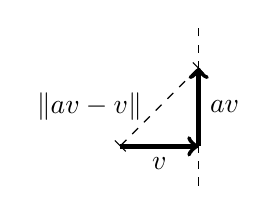
\begin{tikzpicture}
\draw[-, dashed] (1,-.5) -- (1,1.5);
\draw[ultra thick,->] (0,0) -- (.5,0) node[below] {$v$} -- (1,0);
\draw[ultra thick,->] (1,0) -- (1,.5) node[right] {$av$} -- (1,1);
\draw[dashed,|-|] (0,0) -- (.5,.5) node[above, left]{$\|av-v\|\;$} -- (1,1);
\end{tikzpicture}
\end{figure}

\begin{itemize}
\item[$\Rightarrow$] Using Pythagorean Theorem (6.3) $\inner{u,av}=\bar{a}\inner{u,v}=0$ then $\|u+av\|^2 = \|u\|^2+\|av\|^2 \geq \|u\|^2$
\item[$\Leftarrow$]$\|u\|^2 \leq \|u+av\|^2 = \|u\|^2+\|av\|^2 +2\mathrm{Re}\inner{u,av}$. The inequality is not satisfied for all values of $a$ except if the last term vanishes. \hilight{??}
\end{itemize}
%------------------------------------------------------------------------ 
\exo{} Take the vectors $u,v\in\mathbf{R}^n$ such that $u=(a_1, \sqrt{2}a_2, \cdots, \sqrt{n}a_n)$ and  $v=(b_1,b_2/\sqrt{2}, \cdots, b_n/\sqrt{n})$ then using Cauchy-Schwarz (T6) squared leads to
\begin{align*}
|\inner{u,v}|^2 = \left(\sum \sqrt{i}a_ib_i/\sqrt{i}\right)^2 \leq\sum \left(\sqrt{i}a_i\right)^2 \sum\left(b_i/\sqrt{i}\right)^2 = \|u\|^2  \|v\|^2
\end{align*}

%------------------------------------------------------------------------ 
\exo{} Using \eqref{itm:T6_parallelogram_equality} $\|v\|=\sqrt{\frac{\|u+v\|^2 +\|u-v\|^2}{2} - \|u\|^2} =\sqrt{17}$

%------------------------------------------------------------------------ 
\exo{} Let $x\in\mathbf{R}^2$ and $\|x\| = \|(x_1,x_2)\| = |x_1| + |x_2|$ $\stackrel{?}{\implies}$\footnote{Notice that if $\exists \inner{\cdot} \implies \|\cdot\| = \sqrt{\inner{\cdot}}$ but a norm can be defined without an inner product.}$\exists \inner{\cdot}$ such that $\inner{x,x} = \|x\|^2$

\begin{figure}[h!]
\centering
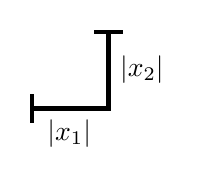
\begin{tikzpicture}
\draw[ultra thick,|-|] (0,0) -- (.5,0) node[below] {$|x_1|$} -- (1,0) -- (1,.5) node[right] {$|x_2|$} -- (1,1);
\end{tikzpicture}
\caption{6.5}
\end{figure}

The inner product can be expressed, using the results of exo.1, as
\begin{align*}
\inner{x,y} = \|x\|\|y\|\cos\theta = \left(|x_1| + |x_2|\right)\left(|y_1| + |y_2|\right)\cos\theta
\end{align*}
which clearly does not satisfy the property of additivity on first slot. Therefore, there is NO inner-product associated to this norm.\\
As a counterexample, let $x=(1,0)$, $y=(0,1)$, $z=(1,1)$, then
\begin{align*}
\inner{x+y,z} &= \left(|x_1+y_1| + |x_2+y_2| \right)\left(|z_1|+|z_2|\right)\cos0 = 4 \\
\inner{x,z} &= \left(|x_1| + |x_2| \right)\left(|z_1|+|z_2|\right)\cos\pi/4 = \sqrt{2} \\
\inner{y,z} &= \left(|y_1| + |y_2| \right)\left(|z_1|+|z_2|\right)\cos\pi/4 = \sqrt{2} 
\end{align*}


%------------------------------------------------------------------------ 
\exo{} If $u,v\in V$ a real inner product space
\begin{align*}
\Aboxed{
\frac{\|u+v\|^2-\|u-v\|^2}{4}= \mathrm{Re}\inner{u,v} = \inner{u,v}}
\end{align*}

%------------------------------------------------------------------------ 
\exo{} If $u,v\in V$ is a complex inner-product space then last equation in previous exercise defining the real part applies. The imaginary part is obtained as
\begin{align*}
\Aboxed{\frac{\|u+\mathrm{j}v\|^2-\|u-\mathrm{j}v\|^2}{4}=\mathrm{Im}\inner{u,v}}
\end{align*}
since 
\begin{align*}
\inner{u,\mathrm{j}v} + \inner{\mathrm{j}v, u}= -\mathrm{j} \underbrace{\left( \inner{u,v} - \overline{\inner{u,v}} \right)}_{2\mathrm{jIm}\mathrm{\inner{u,v}}} = 2\mathrm{Im}\mathrm{\inner{u,v}}
\end{align*}

%------------------------------------------------------------------------ 
\exo{}\label{exo:6_8} if $\|\|:U\to[0,\infty)$ is a norm satisfying \ref{itm:T6_parallelogram_equality} 
$\implies$ $\exists \inner{,}$ on U such that $\|u\|^2 = \inner{u,u}$  $\forall u\in U$.
 
\hilight{TODO}
%------------------------------------------------------------------------ 
\exo{} Let us denote these functions as $k, s_i, c_i$ for the constant, sinus and cosinus vectors. The norms are \begin{align*}
\inner{k,k}&= 1 \\
\inner{s_i,s_i} &= \frac{1}{\pi}\int\limits_0^{\pi}(1 - \cos{2ix})\;dx = \frac{1}{\pi}\left( x - \frac{\sin{2ix}}{2i}\right)\Big|_0^\pi = 1 \\
\inner{c_i,c_i} &=\frac{1}{\pi}\int\limits_0^{\pi}(1 + \cos{2ix})\;dx = 1
\end{align*}
and the inner-products among them
\begin{align*}
\inner{k,s_i}&\propto \int\limits_{-\pi}^\pi \sin{ix}\propto \cos{ix}\Big|_{-\pi}^\pi = 0 &
\inner{k,c_i}&\propto \int\limits_{-\pi}^\pi \cos{ix} \propto \sin{ix}\Big|_{-\pi}^\pi= 0 \\
\inner{s_i,s_j}&\propto \int\limits_{-\pi}^\pi \cos{\Sigma x} - \cos{\Delta x}   = 0&
\inner{c_i,c_j}&\propto \int\limits_{-\pi}^\pi \cos{\Sigma x} + \cos{\Delta x}  = 0\\
\inner{c_i,s_j}& \propto \int\limits_{-\pi}^\pi \sin{\Sigma x} - \sin{\Delta x} = 0 
\end{align*}
where $\Sigma = i+j$ and $\Delta = i-j$ are integers.
%------------------------------------------------------------------------ 
\exo{} $(1,x,x^2)$ are linearly independent in vector space $\mathcal{P}_2(x)$. Applying \ref{itm:T6_gram_schmidt}
\begin{align*}
e_1 &= 1 \\
e_2 &= \frac{x - \inner{x,1} 1 }{\|\star\|} =  \frac{x - 1/2 }{\|\star\|} = \sqrt{3}(2x - 1) \\
e_3 &= \frac{x^2 - \inner{x^2,1} 1 - 3\inner{x^2,2x - 1}(2x - 1)}{\|\circ\|} = \frac{x^{2} - x + \frac{1}{6}}{\|\circ\|} = 6 \sqrt{5} \left(x^{2} - x + \frac{1}{6}\right)
\end{align*}
where
\begin{align*}
\|\star\|^2 &= \int\limits_0^1(x - 1/2)^2\;dx = 1/12 \\
\inner{x^2,2x-1} &= 2\inner{x^2,x} - \inner{x^2,1} = 1/6 \\
\|\circ\|^2 &= \int\limits_0^1\left( x^{2} - 12 x + \frac{17}{3}\right)^2\;dx = \frac{5}{30^2}
\end{align*}


%------------------------------------------------------------------------ 
\exo{} Using \eqref{itm:T6_gram_schmidt} on the first vector that is in the span of the previous vectors will result in the null vector. \\
Specifically. Given a list $(v_1,\cdots, v_n)$ and $v_i \in\mathrm{span}{(v_1,\cdots, v_{i-1})}$ then
\begin{align*}
v_i -\inner{v_i,e_1}e_1 - \cdots -\inner{v_i,e_{i-1}}e_{i-1} = 0 
\end{align*}
Therefore, eliminating the null vectors, GS reduces the original list.

%------------------------------------------------------------------------ 
\exo{}
\hilight{TODO}

%------------------------------------------------------------------------ 
\exo{} \begin{itemize}

\item[$\Leftarrow$] Expanding with orthonormal vectors $v=\sum a_i e_i$ with $a_i=\inner{v,e_i}$ leads to a norm 
\begin{align*}
\|v\|^2 = \inner{v,v} = \sum\limits_i a_i \inner{e_i, \sum\limits_j a_je_j}=\sum\limits_i a_i \sum\limits_j \overline{a_j} \inner{e_i,e_j} = \sum\limits_{ij} a_i \overline{a_j} \delta_{ij}= \sum\limits_i |a_i|^2
\end{align*}

\item[$\Rightarrow$] Let $v\in V$ with $\|v\|^2=\sum |a_i|^2$. 
We start the demonstration finding a basis of $V$ by extending the list of orthogonal vectors with linearly independent vectors $(e_1, \cdots, e_n, u_1, \cdots , u_m)$. Then, we can then express $v=\sum\limits_ja_je_j + u$ where $a_j=\inner{v,e_j}$ and $u$ represents the linear combination with the remaining vectors. Computing now the norm leads to
\begin{align*}
\|v\|^2 = \inner{v,v} = \sum\limits_i |a_i|^2 + 2\mathrm{Re}\sum\limits_ib_i\inner{e_i, u} +\|u\|^2
\end{align*}
which in comparison with the initial expression implies that $u=0$ for arbitrary different values of $e_i$. This leaves in the initial expansion only the orthonormal vectors, i.e. $v\in\mathrm{span}(e_1,\cdots,e_n)$
\end{itemize}
%------------------------------------------------------------------------ 
\exo{}
\hilight{TODO}

%------------------------------------------------------------------------ 
\exo{} Using T29 $V = U\oplus U^\perp$ then $\dim{V} =  \dim{U} + \dim{U^\perp} $

%------------------------------------------------------------------------ 
\exo{}
\begin{itemize}
\item[$\Rightarrow$] if $U^\perp = \{0\}$ then by T33 $(U^\perp)^\perp = U =\{0\}^\perp$. Since any vector is orthogonal to $0$ then $\{0\}^\perp= V$.
\item[$\Leftarrow$] By T29 $V = U \oplus U^\perp$ then substituting $U$ we get  
$V = V \oplus U^\perp$ which means than  $U^\perp=\{0\}$
\end{itemize}


%------------------------------------------------------------------------ 
\exo{} $P\in\mathcal{L}(V)$ and $P^2=P$ then $V = \nullspace{P} \oplus \rangespace{P}$ (see \exref{exo:5_21}). Now here we consider $\nullspace{P} = \rangespace{P}^\perp $ then 
$V = \rangespace{P} \oplus (\rangespace{P})^\perp$. In other words, $P$ map is an orthogonal projection of $V$ onto a subspace $U$ ($= \rangespace{P}$).

%------------------------------------------------------------------------ 
\exo{}

\hilight{TODO}

%------------------------------------------------------------------------ 
\exo{} $\forall u\in U$ a subspace of $V$ and $T\in\mathcal{L}(V)$:
\begin{itemize}
\item[$\Rightarrow$] $u$ and $Tu\in U$ then $P_UTP_Uu = P_UTu = Tu = TP_Uu$ therefore $P_UTP_U = TP_U$.
\item[$\Leftarrow$] $Tu = TP_Uu = P_U T P_Uu = P_U Tu \in U $ therefore $U$ invariant under $T$.
\end{itemize}
%------------------------------------------------------------------------ 
\exo{} Let $u\in U$, $w\in U^\perp$ and therefore $v = u+w \in V$
\begin{itemize}
\item[$\Rightarrow$] $P_UTv = P_UTu + P_UTv= Tu + 0$ since $Tu\in U$ and $Tv \in U^\perp$. Now $P_UTv = Tu = TP_U u$ $\forall u$ so $P_UT = TP_U$.
\item[$\Leftarrow$] $TP_Uv = P_UTv \in U$ and $TP_Uv = Tu$ which means that $Tu\in U$ (i.e. $U$ invariant under $T$). On the other hand, taking $w\in U^\perp$, $P_UTw = TP_Uw = T0 = 0$ which implies that $Tw\in U^\perp$. 
\end{itemize}
The trick is that $U$ is always invariant under $P_U$.

%------------------------------------------------------------------------ 
\exo{} $U=\mathrm{span}\{u_1=(1,1,0,0),u_2=(1,1,1,2)\}$ subspace of $\mathbf{R}^4$: find $u\in U$ that minimizes $\|v-u\|$ with $v=(1,2,3,4)$. 
The solution to this problem consists on mapping $v$ through the orthogonal projection of $V$ onto $U$: $u=P_Uv$ (P36). See that we can decompose v as the sum of elements in two orthogonal subspaces ($U$ and its orthogonal complement)
\begin{align*}
v = \underbrace{\alpha_1 u_1 + \alpha_2 u_2}_{\in U} + \underbrace{w}_{\in U^\perp} = P_U v + w \\
\end{align*}
then projecting on each base of $U$
\begin{align*}
\inner{v,u_1} &= \alpha_1 \|u_1\|^2 + \alpha_2 \inner{u_2,u_1} = 2\alpha_1 + 2\alpha_2 = 3 \\
\inner{v,u_2} &= \alpha_1 \inner{u_2,u_2} + \alpha_2  \|u_2\|^2 =2\alpha_1 + 7\alpha_2 = 14
\end{align*}
which leads to $\alpha_1=-7/10$ and $\alpha_2=11/5$. This means that the closes vector is $u=(1.5,1.5,2.2,4.4)$ which is $\|u-v\| \approx 6.5$.

\hilight{Results in notebook are not minimal!!??}

Another way to do this is to orthonormalize first with GS and then simply project to get the coefficients for every term. But would like to do it with non-orthonormal basis for once.

%------------------------------------------------------------------------ 
\exo{} 
Given $q(x)=2+3x$, find $p$ such that $\|p-q\|^2 = \int\limits_0^1|p(x)-q(x)|^2 dx$ is minimal. But $p$ has further constraints: If $p\in \mathcal{P}_3(x)$ and $p(0)=p'(0)=0$ means that $p(x)=a_2x^2+a_3x^3 = x^2(a_2+a_3x)$ or $p(x)\in U=\mathrm{span}(x^2, x^3)$.

In order to compute the solution solution $P_Uq$ (P36), we will proceed as follows:
\begin{itemize}
\item Obtain orthonormal basis for $U$ $(e_1, e_2)$ using Gram-Schmidt:
\begin{align*}
e_1 &= \sqrt{5}x^2 \\
e_2 &= 6 \sqrt{7} \left(x^{3} - \frac{5 x^{2}}{6}\right)
\end{align*}

\item The minimum is given by $p_\mathrm{min} = P_Uq = \inner{q,e_1}e_1 + \inner{q,e_2} e_2$
\begin{align*}
 P_Uq(x) = - \frac{203 x^{3}}{10} + 24 x^{2}
\end{align*}
\end{itemize}

\begin{figure}[!ht]
\centering
\includegraphics[scale=0.6]{notebooks/21a.pdf} 
\end{figure}

And $\int\limits_0^1|P_Uq(x)-q(x)|^2 dx = 133/100$.

%------------------------------------------------------------------------ 
\exo{}  
After \ref{itm:T6_gram_schmidt}
\begin{align*}
e_0 &= \frac{1}{\sqrt{2\pi}} \\
e_1 &= \frac{\sqrt{6} x}{2 \pi^{\frac{3}{2}}} \\
e_2 &= \frac{\sqrt{10}}{4 \pi^{\frac{5}{2}}} \left(3 x^{2} - \pi^{2}\right) \\
e_3 &= \frac{\sqrt{14} x}{4 \pi^{\frac{7}{2}}} \left(5 x^{2} - 3 \pi^{2}\right) \\
e_4 &= \frac{3 \sqrt{2}}{16 \pi^{\frac{9}{2}}} \left(35 x^{4} - 30 \pi^{2} x^{2} + 3 \pi^{4}\right) \\
e_5 &= \frac{\sqrt{22} x}{16 \pi^{\frac{11}{2}}} \left(63 x^{4} - 70 \pi^{2} x^{2} + 15 \pi^{4}\right) \\
\end{align*}

\begin{figure}[h!]
\centering
\includegraphics[scale=0.8]{notebooks/22a.pdf} 
\end{figure}

Then $u(x)=P_U \sin(x) = \sum_i \inner{e_i,sin(x)}e_i$ which results in:
\begin{align*}
u(x) &= \frac{x}{8 \pi^{10}} \left(- 28 \pi^{4} \left(- \pi^{2} + 15\right) \left(5 x^{2} - 3 \pi^{2}\right) + 11 \left(- 105 \pi^{2} + \pi^{4} + 945\right) \left(63 x^{4} - 70 \pi^{2} x^{2} + 15 \pi^{4}\right) + 24 \pi^{8}\right) \\ 
&= 0.00564311797634677 x^{5} - 0.155271410633428 x^{3} + 0.987862135574673 x
\end{align*}


%------------------------------------------------------------------------ 
\exo{}  
\begin{align*}
p(\frac{1}{2}) &= \int\limits_0^1p(x)q(x)\mathrm{d}x \\
\int\limits_0^1p(x)\delta(x-\frac{1}{2})\mathrm{d}x &=  \inner{p,q} \\
\varphi(p) &= \inner{p,q}
\end{align*}
so using T45, the solution is $q = \sum\limits_{i=0}^2 \varphi(e_i) e_i = $ where $\{e_i\}$ is an orthonormal base in $\mathcal{P}_2(\mathbf{R})$
\begin{align}\label{eq:p2_othn_base}
e_0 &= 1 \\
e_1 &= 2 \sqrt{3} \left(x - \frac{1}{2}\right) \\
e_2 &= 6 \sqrt{5} \left(x^{2} - x + \frac{1}{6}\right) \\
\end{align}

\begin{figure}[h!]
\centering
\includegraphics[scale=0.8]{notebooks/24a.pdf}
\caption{$e_i$ \eqref{eq:p2_othn_base}} 
\end{figure}

In this case $\varphi(e_i) = \int\limits_0^1e_i(x)\delta(x-\frac{1}{2})\mathrm{d}x = e_i(\frac{1}{2})$ so
\begin{align*}
q(x) = - 15 x^{2} + 15 x - \frac{3}{2}
\end{align*}

To test this result, we created an arbitrary vector
\begin{align*}
p(x) = 0.512524207064677 x^{2} + 0.114279229148524 x + 0.157036682514979 \in  \mathcal{P}_2(\mathrm{R})
\end{align*}
and
\begin{align*}
p\left(\frac{1}{2}\right) &= \int\limits_0^1p(x)q(x)\mathrm{d}x = 0.342307348855410
\end{align*}

\begin{figure}[h!]
\centering
\includegraphics[scale=0.8]{notebooks/24b.pdf}
\caption{6.24 $p$ (red) and $q$ (blue)} 
\end{figure}

Some thoughts:
\begin{itemize}
\item $\int_a^b q(x)p(x)\mathrm{d}x/(b-a)= \int_0^1 q(x)p(x)\mathrm{d}x$ can be seen as a weighted average of $p$ in the interval $[0,1]$.  
\item Mean value theorem claims that the result of this integral is the function evaluated at some point within the interval: $\int_0^1 q(x)p(x)\mathrm{d}x = p(c)$. Roughly speaking the function passes through its mean at some point in the interval.
\item Therefore, this problem can be seen as finding the weight function $q(x)$ such that the weighted mean of any polynomial $p(x)$ corresponds to its point at $x=1/2$.
\item I would expect this function to "modulate" $p(x)$ such that the new function $p(x)q(x)$ has a mean value equal $p(1/2)$. Therefore one could expect that the construction of $q(x)$ depends on the shape of $p(x)$ ... but the linear functional does not incorporates this dependency!??
\end{itemize}


%------------------------------------------------------------------------ 
\exo{} This problem is resolved using the same bases as in the previous exercise but targeting a different linear functional on $\mathcal{P}_2(\mathbf{R})$:
\begin{align*}
\varphi(p) = \int\limits_0^1p(x)\cos(\pi x)\mathrm{d}x = \inner{p,q} 
\end{align*}
Using an analogous procedure, the resulting vector $q\in\mathcal{P}_2(\mathbf{R})$ is
\begin{align}
\label{eq:res25a}
q(x)= - \frac{1}{\pi^{2}} \left(24 x - 12\right)
\end{align}
Testing with $p(x)= 0.891160980850087 x^{2} + 0.816413394341083 x + 0.970635204024762$ we obtain
\begin{align*}
\varphi(p) = \inner{p,q} = -0.346026913703390
\end{align*}

\begin{figure}[h!]
\centering
\includegraphics[scale=0.8]{notebooks/25a.pdf}
\caption{ exo 6.25 $q$ (red) and test function $p$ (blue) }
\end{figure}

%------------------------------------------------------------------------ 
\exo{} By the definition of adjoint of $T\in \mathcal{L}(V,\mathbf{F})$ $\inner{Tu, a}=\inner{u, T^*a}$. Developing the first term
\begin{align*}
\inner{Tu, a} = \overline{a}\inner{Tu, 1} = \overline{a}Tu = \overline{a}\inner{u,v} = \inner{u,av}
\end{align*}
and since $T^*a$ is a unique choice, then $T^*a = av$

\hilight{Not sure about $\inner{Tu, 1}$}
%------------------------------------------------------------------------ 
\exo{}  
\begin{align*}
\inner{Tz,w} = z_1w_2 + \cdots z_{n-1}w_n = \inner{z, T^*w}
\end{align*}
and therefore $T^*w = (w_2,\cdots, w_n, 0)$ \qed \\

For the sake of simplicity, take $n=3$, then for standard basis
\begin{align*}
\mathcal{M}(T) = \begin{bmatrix}
0 & 0 & 0 \\
1 & 0 & 0 \\
0 & 1& 0
\end{bmatrix}
&&
\mathcal{M}(T^*) = \mathcal{M}(T)^H = \begin{bmatrix}
0 & 1 & 0 \\
0 & 0 & 1 \\
0 & 0& 0
\end{bmatrix}
\end{align*}
which $\mathcal{M}(T^*)(a_1,a_2,a_2) = (a_2, a_3, 0)$

%------------------------------------------------------------------------ 
\exo{\label{exo:6_28}}  
\begin{align*}
\inner{Tu,w} = \inner{\lambda u,w} = \inner{u,\overline{\lambda}w} =  \inner{u,T^*w}
\end{align*}
Because according to the definition of \ref{itm:D6_adjoint}, the vector on the right-hand side is unique and therefore $T^*w = \overline{\lambda}w$.

%------------------------------------------------------------------------ 
\exo{} Let $T\in\mathcal{L}(V)$ and $U$ subspace of $V$:
\begin{align*}
\forall u\in U \quad Tu\in U \iff \forall w\in U^\perp \quad T^*w\in U^\perp
\end{align*}

\begin{enumerate}
\item[$\Rightarrow$)] $Tu\in U \implies \inner{Tu,w}=0$ since $w\in U^\perp$. It also $\exists!T^*w\in V$ such that $\inner{Tu,w}=\inner{u,T^*w}$. Therefore $\inner{u,T^*w}=0 \implies T^*w\in U^\perp$ \qed
\item[$\Leftarrow$)] Analogously, given $T^*w\in U^\perp$ and $u\in U$ then $\inner{T^*w,u} = \inner{w, T^{**}u} = \inner{w, Tu} = 0 \implies Tu\in U^{\perp\perp}=U$, where we have used the adjoint of adjoint property of $T\to T^*$ and C.30.
\end{enumerate}

%------------------------------------------------------------------------ 
\exo{} Let $T\in\mathcal{L}(V,W)$. 
\begin{align*}
T\; \textrm{injective/surjective} \iff T^*\; \textrm{surjective/injective}
\end{align*}
To demonstrate this we will use P3.2, P.46 and C.30:
\begin{enumerate}
\item[$\Rightarrow$)] $T$ injective $\iff \nullspace{T} = \{0\} = (\rangespace{T^*})^\perp \implies \rangespace{T^*} = \{0\}^\perp = V$ therefore $T^*$ is surjective.\\
$T$ surjective $\iff \rangespace{T} = V = (\nullspace{T^*})^\perp \implies \nullspace{T^*} = V^\perp = \{0\}$ therefore $T^*$ is injective.
\item[$\Rightarrow$)] Analogously, by interchanging $T$ and $T^*$.

\end{enumerate}

%------------------------------------------------------------------------ 
\exo{} Here we will use the relations in \ref{itm:P6_46} with two more properties: The first is the property that allows us to express a vector space as a direct sum of a subspace and its orthogonal complement $V = U\oplus U^\perp$ 
\begin{align*}
\dim{V} &= \dim{\nullspace{T}} + \dim{(\nullspace{T})^\perp} \\&=  \dim{\nullspace{T}} + \dim{\rangespace{T^*}} \\
\dim{W} &= \dim{\nullspace{T^*}} + \dim{(\nullspace{T^*})^\perp} \\&= \dim{\nullspace{T^*}} + \dim{\rangespace{T}}
\end{align*}
and the theorem 3.4 for a linear map $T\in\mathcal{L}(V,W)$:
\begin{align*}
\dim{V} &= \dim{\nullspace{T}} + \dim{\rangespace{T}} \\
\dim{W} &= \dim{\nullspace{T^*}} + \dim{\rangespace{T^*}}
\end{align*}
Subtracting two of the four expressions shows that
\begin{align*}
\Aboxed{\dim{\rangespace{T}} = \dim{\rangespace{T^*}}}
\end{align*}
Finally using the latter and subtracting the outcome of T3.4
\begin{align*}
\dim{V} - \dim{W} &= \dim{\nullspace{T}} - \dim{\nullspace{T^*}}
\end{align*} 
\qed
%------------------------------------------------------------------------ 
\exo{} Given row vectors $r_1,\cdots,r_m\in\mathbf{R}^n$ and column vectors $c_1,\cdots,r_n\in\mathbf{R}^m$ of a real $m\times n$ matrix $A$, we need to proof that
\begin{align*}
\dim{\mathrm{span}(c_1,\cdots,c_n)} = \dim{\mathrm{span}(r_1,\cdots,r_m)}  
\end{align*}

Let define $A = \mathcal{M}\left(T, (e_1,\cdots, e_n), (f_1,\cdots, f_m)\right)$ with $T\in\mathcal{L}(\mathbf{R}^n, \mathbf{R}^m)$. By P2.8, every spanning set of vectors $(c_1,\cdots,c_n)\in\mathbf{R}^m$ can be reduced to basis in $\mathbf{R}^m$:
\begin{align*}
\mathrm{span}(c_1,\cdots,c_n) = \mathrm{span}(Te_1,\cdots,Te_n) =  \mathrm{span}(f_1,\cdots,f_p) = \rangespace{T}
\end{align*}
where $p\leq n$ (is a reduction) and $p\leq m$ (cannot be greater that the dimension of $\mathbf{R}^m$). 
According to P47, $A^T = \mathcal{M}\left(T^*, (f_1,\cdots, f_m), (e_1,\cdots, e_n))\right)$. Following an analogous approach
\begin{align*}
\mathrm{span}(r_1,\cdots,r_m) = \mathrm{span}(T^*f_1,\cdots,T^*f_m) =  \mathrm{span}(e_1,\cdots,e_p) = \rangespace{T^*}
\end{align*}
with $q\leq m$ and $q\leq n$. Finally, since $\dim{\rangespace{T}} = \dim{\rangespace{T^*}}$ (from previous exercise) we demonstrate that $p = q$. \qed

\begin{figure}[htbp!]
\label{fig:adjoint_map}
\centering
\includegraphics[scale=0.5, clip, trim=0cm 4cm 1cm 1cm]{figs/Adjoint.pdf}
\caption{Adjoint map: Notice that the subspaces in the direct sum they are as well orthogonal.} 
\end{figure}


